\section{Logical Design}

\subsection{Volume Table}
Lets consider the volumes for a year

\begin{table}[H]
    \scriptsize
    \renewcommand{\arraystretch}{1.3} % Adjust row height
    \begin{tabularx}{\textwidth}{|X|X|X|X|}
    \hline
    \textbf{Concept}& \textbf{Type}  & \textbf{Volume}    & \textbf{Description}     \\ \hline
    Facility & E & 100 & Number of facilities (Given) \\ \hline
    Contract & E & 900.000 & Number of contracts. 100 facilities * 500 contracts per facility * 12 months * 1.5 contracts per account \\ \hline
    Customer & E & 300.000 & Number of customers.(ASSUMPTION) \\ \hline
    Account & E & 600.000 & Number of accounts. 300.000 customers * 2 accounts per customer on average\\ \hline
    Team & E & 50 & Number of teams. (Given) \\ \hline
    Employee & E & 250 & Number of employees. 5 employees per team * 100 teams (ASSUMPTION) \\ \hline
    Feedback & E & 600.000 & Number of feedbacks.\\ \hline
    Provides & R & 900.000 & Each contract is provided by a single facility \\ \hline
    Linked & R & 900.000 & On average each account has 1.5 contracts \\ \hline
    Has & R & 600.000 & Each customer 2 accounts on average \\ \hline
    OverseenBy & R & 100 & Each facility is overseen by a single team. Each team oversees 2 facilities, on average \\ \hline
    Configuration & R & 500 & Each team constists of 5 employees on average \\ \hline
    Gives & R & 500.000 & Each feedback is given by a single account.Not all accounts give feedback  \\ \hline
    Evaluation & R & 500.000 & Each feedback is linked to a single team\\ \hline
    \end{tabularx}
    \caption{Volume Table}
\end{table}

\subsection{Access Table}

\textbf{Operation1:} Register a new customer (50 times per day)\\
\begin{table}[H]
    \renewcommand{\arraystretch}{1.3} % Adjust row height
    \begin{tabularx}{\textwidth}{|X|X|X|X|}
    \hline
    \textbf{Concept}& \textbf{Type}  & \textbf{Access}    & \textbf{Type}     \\ \hline
    Customer & E & 1 & W \\ \hline
    \end{tabularx}
    \caption{Access Table for Operation1}
\end{table}
\noindent Total Cost: 2 * 50 = 100 per day
\newline
\textbf{Operation2:} Register a new energy contract (50 times per day)\\
\begin{table}[H]
    \renewcommand{\arraystretch}{1.3} % Adjust row height
    \begin{tabularx}{\textwidth}{|X|X|X|X|}
    \hline
    \textbf{Concept}& \textbf{Type}  & \textbf{Access}    & \textbf{Type}     \\ \hline
    Contract & E & 1 & W \\ \hline
    Provides & R & 1 & W \\ \hline
    Facility & E & 1 & R \\ \hline
    Linked & R & 1 & W \\ \hline
    Account & E & 1 & R \\ \hline
    Facility & E & 1 & W \\ \hline
    Provides & R & 9000 & R \\ \hline
    Contract & E & 9000 & R \\ \hline
    \end{tabularx}
    \caption{Access Table for Operation2}
\end{table}
\noindent Total Cost: (2+2+1+2+1+2+9000+9000)*200=3.602.000 per day

\noindent Every time we need to update the efficiency score of the facility related to the contracts.
\newline
\noindent \textbf{Operation3:} Assign a facility to a management team (50 times per day)\\
\begin{table}[H]
    \renewcommand{\arraystretch}{1.3} % Adjust row height
    \begin{tabularx}{\textwidth}{|X|X|X|X|}
    \hline
    \textbf{Concept}& \textbf{Type}  & \textbf{Access}    & \textbf{Type}     \\ \hline
    Team & E & 1 & R \\ \hline
    OverseenBy & R & 1 & W \\ \hline
    Facility & E & 1 & R \\ \hline
    \end{tabularx}
    \caption{Access Table for Operation3}
\end{table}
\noindent Total Cost: (1+2+1)*50=200 per day
\newline
\noindent \textbf{Operation4:} View the total energy output of a specific facility managed by the eldest employee (1 per month = 0.03 per day)\\
\begin{table}[H]
    \renewcommand{\arraystretch}{1.3} % Adjust row height
    \begin{tabularx}{\textwidth}{|X|X|X|X|}
    \hline
    \textbf{Concept}& \textbf{Type}  & \textbf{Access}    & \textbf{Type}     \\ \hline
    Employee & E & 250 & R \\ \hline
    Configuration & R & 1 & R \\ \hline
    Team & E & 1 & R \\ \hline
    OverseenBy & R & 2 & R \\ \hline
    Facility & E & 2 & R \\ \hline
    Provides & R & 9000 & R \\ \hline
    Contract & E & 9000 & R \\ \hline
    \end{tabularx}
    \caption{Access Table for Operation4}
\end{table}
\noindent Total Cost: (250+1+1+1+2+9000+9000)*0.03=547.65 per day
\newline
\noindent Each team oversees, on average, twow facilities. We need to choose only one of them, which provides on average 9000 contracts.
In this case we don't have sumEnergyOutput in the schema as attribute of the facility, so we need to compute it every time. If we introduce it, the cost will be
\begin{table}[H]
    \renewcommand{\arraystretch}{1.3} % Adjust row height
    \begin{tabularx}{\textwidth}{|X|X|X|X|}
    \hline
    \textbf{Concept}& \textbf{Type}  & \textbf{Access}    & \textbf{Type}     \\ \hline
    Employee & E & 250 & R \\ \hline
    Configuration & R & 1 & R \\ \hline
    Team & E & 1 & R \\ \hline
    OverseenBy & R & 2 & R \\ \hline
    Facility & E & 2 & R \\ \hline
    \end{tabularx}
    \caption{Access Table for Operation4 with redundancy}
\end{table}
\noindent Total Cost: (250+1+1+2+2)*0.03=7.68 per day
\newline
\noindent But in this case we need to update it every time we add a new contract, so the total cost of \textbf{Operation2} will be:

\begin{table}[H]
    \renewcommand{\arraystretch}{1.3} % Adjust row height
    \begin{tabularx}{\textwidth}{|X|X|X|X|}
    \hline
    \textbf{Concept}& \textbf{Type}  & \textbf{Access}    & \textbf{Type}     \\ \hline
    Contract & E & 1 & W \\ \hline
    Provides & R & 1 & W \\ \hline
    Facility & E & 1 & R \\ \hline
    Facility & E & 1 & W \\ \hline
    Linked & R & 1 & W \\ \hline
    Account & E & 1 & R \\ \hline
    Facility & E & 1 & W \\ \hline
    Provides & R & 9000 & R \\ \hline
    Contract & E & 9000 & R \\ \hline
    \end{tabularx}
    \caption{Access Table for Operation2 with redundancy}
\end{table}
\noindent Total Cost: (2+2+1+2+2+1+2+9000+9000)*200=3.602.400 per day
\newline
\noindent So the total cost without redundancy is 3.602.000 +547.65 = 3.602.547.65, while the total cost with redundancy is 3.602.400 + 7.68 = 3.602.407.68 per day. So we should keep the redundancy in this case. 
\newline
\noindent \textbf{Operation5:} Print a ranked list of facilities based on their efficiency scores (10 per day)
\begin{table}[H]
    \renewcommand{\arraystretch}{1.3} % Adjust row height
    \begin{tabularx}{\textwidth}{|X|X|X|X|}
    \hline
    \textbf{Concept}& \textbf{Type}  & \textbf{Access}    & \textbf{Type}     \\ \hline
    Facility & E & 100 & R \\ \hline
    \end{tabularx}
    \caption{Access Table for Operation5}
\end{table}
\noindent Total Cost: 100*10 = 1000 per day

\noindent We can try to remove the redundancy of the efficiencyScore in facilities
\begin{table}[H]
\renewcommand{\arraystretch}{1.3} % Adjust row height
\begin{tabularx}{\textwidth}{|X|X|X|X|}
\hline
\textbf{Concept}& \textbf{Type}  & \textbf{Access}    & \textbf{Type}     \\ \hline
Facility & E & 100 & R \\ \hline
Provides & R & 900.000 & R \\ \hline
Contract & E & 900.000 & R \\ \hline
\end{tabularx}
\caption{Access Table for Operation5 without redundancy}
\end{table}
\noindent Total Cost: (100+900.000+900.000)*10 = 18.001.000 per day 
\begin{table}[H]
    \renewcommand{\arraystretch}{1.3} % Adjust row height
    \begin{tabularx}{\textwidth}{|X|X|X|X|}
    \hline
    \textbf{Concept}& \textbf{Type}  & \textbf{Access}    & \textbf{Type}     \\ \hline
    Contract & E & 1 & W \\ \hline
    Provides & R & 1 & W \\ \hline
    Facility & E & 1 & R \\ \hline
    Linked & R & 1 & W \\ \hline
    Account & E & 1 & R \\ \hline
    \end{tabularx}
    \caption{Access Table for Operation2 without redundancy}
\end{table}
\noindent Total Cost: (2+2+1+2+1)*200=1.600 per day
\newline
\noindent Now we don't need to update the the efficiency score everytime we register a new contract.

\noindent So the total cost without redundancy is 18.002.600, while the total cost with redundancy is 2.402.000 + 1000 = 2.403.000 per day.

\noindent We shouuld keep the redundancy in this case.

\subsubsection{Redundancies and Generalization}
\begin{itemize}
    \item \textbf{Redundancies:} The number of contracts handled by a team is not stored in the schema, as it can be calculated by counting the number of contracts related to the facility managed by the team. The score of the team can be derived by the following formula: $score = \frac{energy\_efficiency + uptime + AVG(customer\_score)}{3}$ and is not stored in the schema to avoid redundancy. Due to the previous analysis, the redundancy of the efficiency score and sumEngergyOutput in the facility are kept in the schema
    \item \textbf{Generalization:} The schema doesn't contain any generalization since there aren't different operations for theme. There is a \textbf{type} attribute in the \textbf{Customer} and \textbf{Contract} entities so that the business rule related to the type of contract can be enforced.
\end{itemize}


\subsection{UML Schema}

\begin{figure}[H]
    \centering
    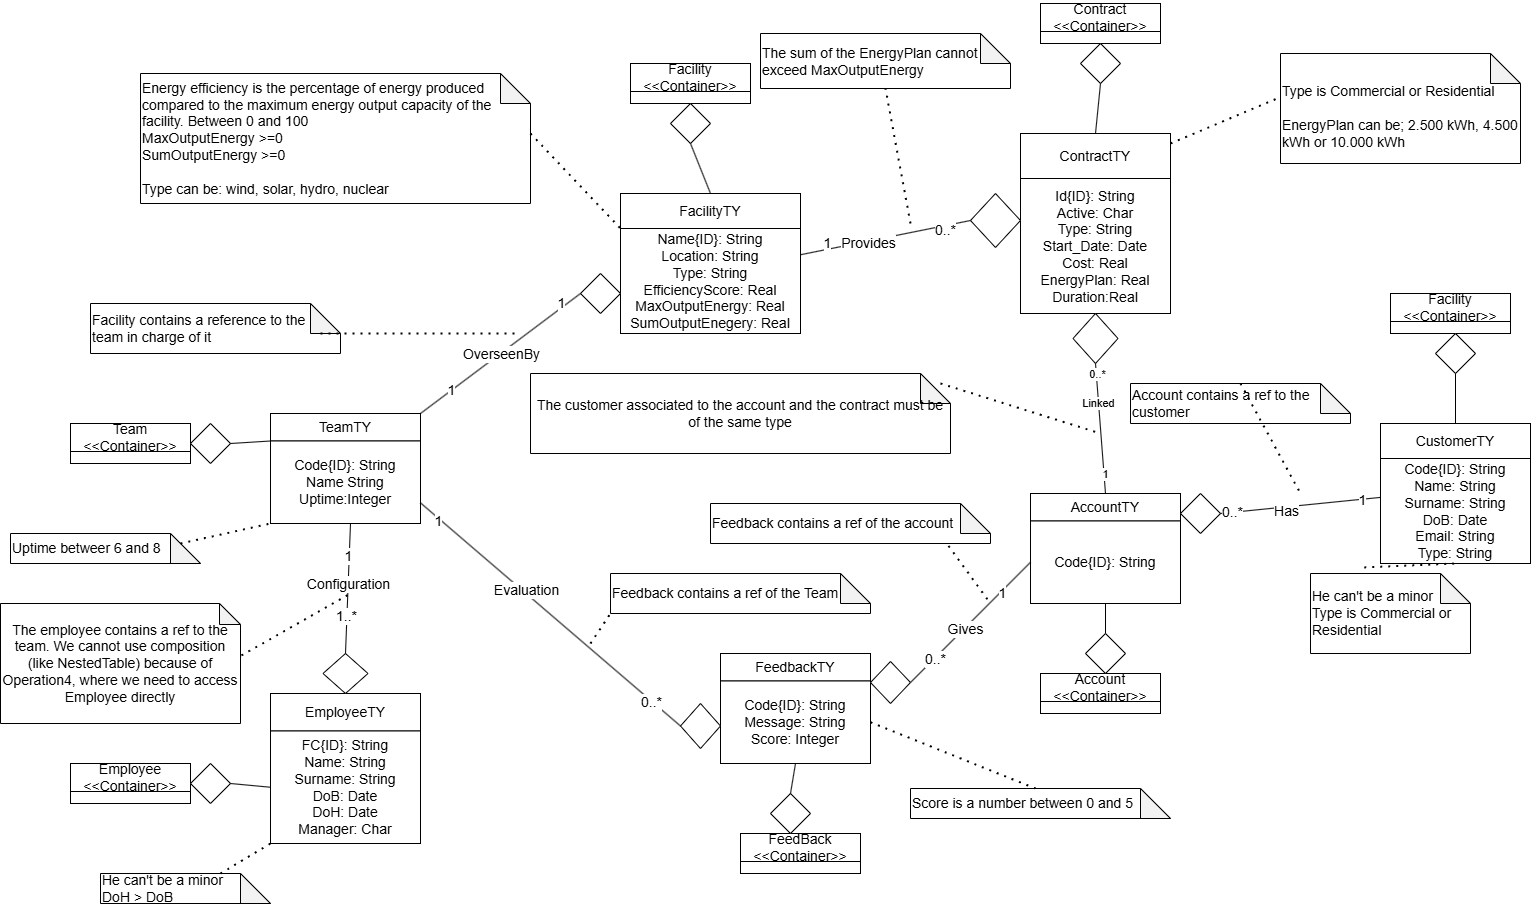
\includegraphics[width=\textwidth]{images/UML.png}
    \caption{UML Schema}
\end{figure}
